\documentclass[11pt,a4paper]{article}

% ----------------------------------------------------------------
% Project Report Preamble
% ----------------------------------------------------------------
\usepackage[margin=1in]{geometry}
\usepackage{amsmath,amssymb,amsthm}
\usepackage{graphicx}
\usepackage{booktabs}
\usepackage{array}
\usepackage{makecell}
\usepackage{longtable}
\usepackage{multirow}
\usepackage{tabularx}
\usepackage{microtype}
\usepackage{url}
\usepackage{xurl}
\usepackage{float}
\usepackage{caption}
\usepackage{subcaption}
\usepackage{hyperref}
\usepackage{xcolor}
\usepackage{enumitem}
\usepackage{fancyhdr}

\hypersetup{
  colorlinks=true,
  linkcolor=blue,
  citecolor=blue,
  urlcolor=blue,
  pdftitle={Project Report: Benchmarking Object Detectors on FathomNet Underwater Imagery},
  pdfauthor={Charan Rasineni}
}

\captionsetup{font=small,labelfont=bf}

\pagestyle{fancy}
\fancyhf{}
\fancyhead[L]{\small Benchmarking Object Detectors on FathomNet Underwater Imagery}
\fancyhead[R]{\small Page \thepage}
\fancyfoot[C]{}
\renewcommand{\headrulewidth}{0.4pt}

\newcommand{\dataset}{\textsc{FathomNet CLEF 2026}}

\begin{document}

% ----------------------------------------------------------------
% TITLE PAGE
% ----------------------------------------------------------------
\begin{titlepage}
\begin{center}
\vspace*{1.5cm}
{\LARGE\bfseries Benchmarking Two-Stage, One-Stage, and Transformer\\
\vspace{0.4cm}
Object Detectors on Under-Sampled Marine Biodiversity Imagery\par}
\vspace{1.2cm}
{\large A Deep Learning Project Report\par}
\vspace{1.6cm}

\begin{tabular}{ll}
\textbf{Student:} & Charan Rasineni \\
\textbf{Program:} & B.Tech, Computer Science and Engineering \\
\textbf{School:} & School of Computer Science and Engineering (SCOPE) \\
\textbf{University:} & VIT-AP University, Amaravati, 522241, India \\
\textbf{Email:} & charan.24bce7827@vitapstudent.ac.in \\[0.6cm]
\textbf{Mentor:} & Dr. Rajesh Duvvuru \\
\textbf{Role:} & Mentor, SCOPE, VIT-AP University \\
\textbf{Email:} & rajesh.duvvuru@vitap.ac.in \\
\end{tabular}

\vfill
\vspace{0.8cm}
{\small \today\par}
\end{center}
\end{titlepage}

% ----------------------------------------------------------------
% ABSTRACT
% ----------------------------------------------------------------
\begin{abstract}
\noindent Automated monitoring of marine biodiversity from remotely operated vehicle (ROV) and autonomous underwater vehicle (AUV) imagery requires object detectors capable of identifying dozens of poorly sampled taxonomic groups under challenging optical conditions. This report presents a controlled benchmark of three representative object detection architectures --- the two-stage Faster R-CNN R50-FPN, the one-stage YOLOv8s, and the end-to-end transformer-based RT-DETR-L --- on the \dataset{} underwater object detection dataset, a community benchmark comprising 5,817 labelled training images and 646 validation images distributed across 32 taxonomic classes with a strongly long-tailed frequency distribution.

All three detectors are trained and evaluated under an identical experimental protocol: the same stratified 90/10 image-level split (seed 42), the same $640\times640$ input resolution, the same COCO-style mean average precision (mAP) evaluation via \texttt{pycocotools}, and the same confidence threshold ($0.001$) and per-image detection cap ($300$). Experiments are conducted on a single NVIDIA T4 GPU with 15~GiB memory.

Faster R-CNN R50-FPN achieves the strongest overall accuracy (mAP$_{50\text{-}95}=0.333$, mAP$_{50}=0.483$), followed by YOLOv8s ($0.313/0.428$) and RT-DETR-L ($0.231/0.323$). YOLOv8s is the fastest detector at $24.0$~ms per image, versus $46.4$~ms for Faster R-CNN and $62.2$~ms for RT-DETR-L. A consistent head-to-tail degradation is observed across all three architectures, reflecting the long-tailed class distribution, and small objects are effectively undetected at the nominal input resolution. These findings provide a practical accuracy--cost--latency trade-off for deploying underwater perception pipelines on ROV/AUV platforms.

\medskip
\noindent\textbf{Keywords:} Object detection; Faster R-CNN; YOLOv8; RT-DETR; underwater imagery; marine biodiversity; FathomNet; long-tailed learning; benchmarking; deep learning.
\end{abstract}

% ----------------------------------------------------------------
% TABLE OF CONTENTS
% ----------------------------------------------------------------
\tableofcontents
\newpage

% ----------------------------------------------------------------
% 1. INTRODUCTION
% ----------------------------------------------------------------
\section{Introduction}
\label{sec:introduction}

The oceans cover more than 70\% of Earth's surface and host a vast fraction of the planet's biodiversity, yet large portions of the deep sea remain poorly explored and documented. Remotely operated vehicles (ROVs) and autonomous underwater vehicles (AUVs) equipped with cameras now routinely collect terabytes of underwater imagery, offering an unprecedented window into marine ecosystems. However, the sheer volume of collected imagery far exceeds the capacity of human experts to annotate and identify organisms manually. Automated object detection --- the task of localizing and classifying instances of interest in images --- is therefore a critical enabling technology for scalable marine biodiversity monitoring.

Underwater object detection is substantially more difficult than terrestrial object detection. Water absorbs and scatters light, causing reduced contrast, colour cast, and limited visibility, particularly at depth. Turbidity, variable illumination, backscatter, occlusion, and biological camouflage further degrade image quality. Many marine taxa are small, rare, or exhibit high intra-class morphological variation, and annotated training data are scarce for most species. These challenges are compounded by extreme class imbalance: a small number of common taxa account for the majority of annotated instances, while numerous rare taxa are represented by only a handful of examples. A detector deployed in this setting must therefore generalize across both frequent ``head'' classes and a long ``tail'' of under-sampled taxa.

Recent years have seen rapid progress in object detection, with three dominant architectural families emerging: two-stage detectors (exemplified by Faster R-CNN~\cite{fasterrcnn2015} and its Feature Pyramid Network~\cite{fpn2017} extension), one-stage dense detectors (exemplified by YOLO~\cite{yolov8_2023}), and end-to-end transformer-based detectors (exemplified by DETR~\cite{detr2020} and RT-DETR~\cite{rtdetr2024}). Each family makes different inductive biases and computational trade-offs, but their relative performance on long-tailed underwater imagery has not been systematically characterized under a controlled protocol.
This report addresses that gap. We benchmark Faster R-CNN R50-FPN, YOLOv8s, and RT-DETR-L on the \dataset{} dataset, a benchmark for underwater object detection drawn from the FathomNet image database~\cite{fathomnet2022} and the ImageCLEF LifeCLEF 2026 track~\cite{fathomnet-clef-2026}. The dataset contains 5,817 labelled training images and 646 validation images spanning 32 taxonomic classes, with a strongly long-tailed annotation distribution in which the three most frequent classes account for 53.4\% of training annotations while the rarest class has only six instances. All models are trained and evaluated under an identical protocol to isolate architectural differences from confounds such as data split, input resolution, and evaluation settings.

The contributions of this work are:
\begin{enumerate}[leftmargin=*]
  \item A controlled, equal-protocol benchmark of a two-stage, one-stage, and transformer detector on \dataset{} underwater imagery.
  \item A head/mid/tail and object-size stratified error analysis revealing where each architecture succeeds and fails.
  \item An accuracy--inference-cost--latency trade-off analysis relevant to deployment on resource-constrained ROV/AUV platforms.
  \item A documented assessment of GPU memory constraints for transformer detectors on commodity hardware (15~GiB T4).
\end{enumerate}

The remainder of this report is organized as follows. Section~\ref{sec:related-work} reviews related work. Section~\ref{sec:dataset} describes the dataset and its properties. Section~\ref{sec:methods} details the detector architectures, experimental protocol, and training setup. Section~\ref{sec:results} presents quantitative and qualitative results. Section~\ref{sec:discussion} discusses the findings, Section~\ref{sec:limitations} outlines limitations, and Section~\ref{sec:conclusion} concludes with future work.

% ----------------------------------------------------------------
% 2. RELATED WORK
% ----------------------------------------------------------------
\section{Related Work}
\label{sec:related-work}

\subsection{Underwater Object Detection}
Underwater vision differs fundamentally from terrestrial computer vision. Light attenuation in water is wavelength-dependent, with red wavelengths absorbed first, yielding a characteristic blue-green colour cast; scattering produces backscatter and reduces contrast; and illumination is often non-uniform due to artificial lighting on ROVs/AUVs. Chen et al.~\cite{underwater-survey} survey underwater object detection in the era of artificial intelligence, identifying turbidity, low contrast, colour distortion, small objects, and class imbalance as the principal challenges. Earlier work on the FathomNet training database demonstrated that large-scale annotated underwater image collections can support the training of accurate deep detectors~\cite{fathomnet-2021-workshop}. The \dataset{} benchmark extends this effort by providing a standardized, community-maintained testbed for underwater object detection~\cite{fathomnet-clef-2026}.

\subsection{Detector Families}

\textbf{Two-stage detectors.} Faster R-CNN~\cite{fasterrcnn2015} introduced the Region Proposal Network (RPN), which shares convolutional features between proposal generation and detection, enabling near real-time two-stage detection. The Feature Pyramid Network (FPN)~\cite{fpn2017} augments this architecture with a top-down pathway and lateral connections, producing strong feature representations at multiple scales --- particularly valuable for small objects. Faster R-CNN with an R50-FPN backbone is a widely used accuracy benchmark in object detection.

\textbf{One-stage detectors.} The You Only Look Once (YOLO) family reformulates detection as a single regression problem, predicting bounding boxes and class probabilities directly from dense anchor points (or anchor-free keypoints in recent versions). YOLOv8~\cite{yolov8_2023}, distributed by Ultralytics~\cite{ultralytics}, balances speed and accuracy through an anchor-free detection head, a CSPDarknet backbone, and efficient training augmentations. The ``s'' (small) variant, YOLOv8s, is designed for resource-constrained deployment while retaining competitive accuracy.

\textbf{Transformer-based detectors.} DEtection TRansformer (DETR)~\cite{detr2020} treats object detection as a set prediction problem, eliminating hand-designed components such as NMS and anchor generation. Deformable DETR~\cite{deformable-detr2021} improves convergence and small-object handling via deformable attention. RT-DETR~\cite{rtdetr2024} is an end-to-end real-time transformer detector that interleaves CNN backbone features with an efficient hybrid encoder and IoU-aware query selection, aiming to combine transformer accuracy with real-time inference. RT-DETR-L denotes the large variant evaluated here.

\subsection{Long-Tailed Recognition}
Long-tailed distributions are common in biodiversity datasets, where a few species dominate observations and most species are rare. Standard cross-entropy training tends to bias detectors toward head classes at the expense of tail classes. Although this report does not propose a new long-tailed algorithm, the head/mid/tail analysis in Section~\ref{sec:results-perclass} quantifies how the architecture-independent data distribution constrains performance across all three detector families.

% ----------------------------------------------------------------
% 3. DATASET
% ----------------------------------------------------------------
\section{The \dataset{} Dataset}
\label{sec:dataset}

\subsection{Scope and Collection}
The \dataset{} dataset is an underwater object detection benchmark built on the FathomNet global image database~\cite{fathomnet2022,fathomnet-2021-workshop} and organized as the ImageCLEF LifeCLEF 2026 underwater object detection track~\cite{fathomnet-clef-2026}. Imagery is collected from ROV and AUV platforms across diverse marine environments. Each image is annotated with bounding boxes and taxonomic labels by domain experts, yielding a multi-class detection benchmark with 32 taxonomic classes spanning invertebrates, fishes, corals, and other marine organisms.

\subsection{Dataset Statistics}
Table~\ref{tab:dataset} summarizes the dataset. The training set comprises 5,817 labelled images and the validation set 646 images, distributed over 32 classes. The annotation distribution is strongly long-tailed: the three most frequent classes (bony fish, brittle star, urchin --- the ``head'' group) account for approximately 53.4\% of all training annotations, while the rarest class contains only six annotated instances. The remaining classes are organized into a ``mid'' group (anemone, sea fan, sponge, stony coral) and a ``tail'' group comprising the other 25 classes.

\begin{table}[H]
\centering
\small
\caption{\dataset{} dataset statistics.}
\label{tab:dataset}
\begin{tabular}{@{}ll@{}}
\toprule
Property & Value \\
\midrule
Training images & 5,817 \\
Validation images & 646 \\
Number of classes & 32 \\
Annotation distribution & Long-tailed \\
Head classes (top 3) & bony fish, brittle star, urchin \\
Mid classes & anemone, sea fan, sponge, stony coral \\
Tail classes & 25 remaining classes \\
Top-3 share of annotations & $\approx$ 53.4\% \\
Rarest class annotation count & 6 \\
\bottomrule
\end{tabular}
\end{table}
Figure~\ref{fig:class-imbalance} visualizes the per-class annotation counts, illustrating the severity of the long tail. The imbalance has direct consequences for detector training: head classes receive dense gradient signal, whereas tail classes are under-represented and prone to being missed entirely (several tail classes achieve zero average precision across all three detectors, as shown in Section~\ref{sec:results-perclass}).

\begin{figure}[H]
\centering
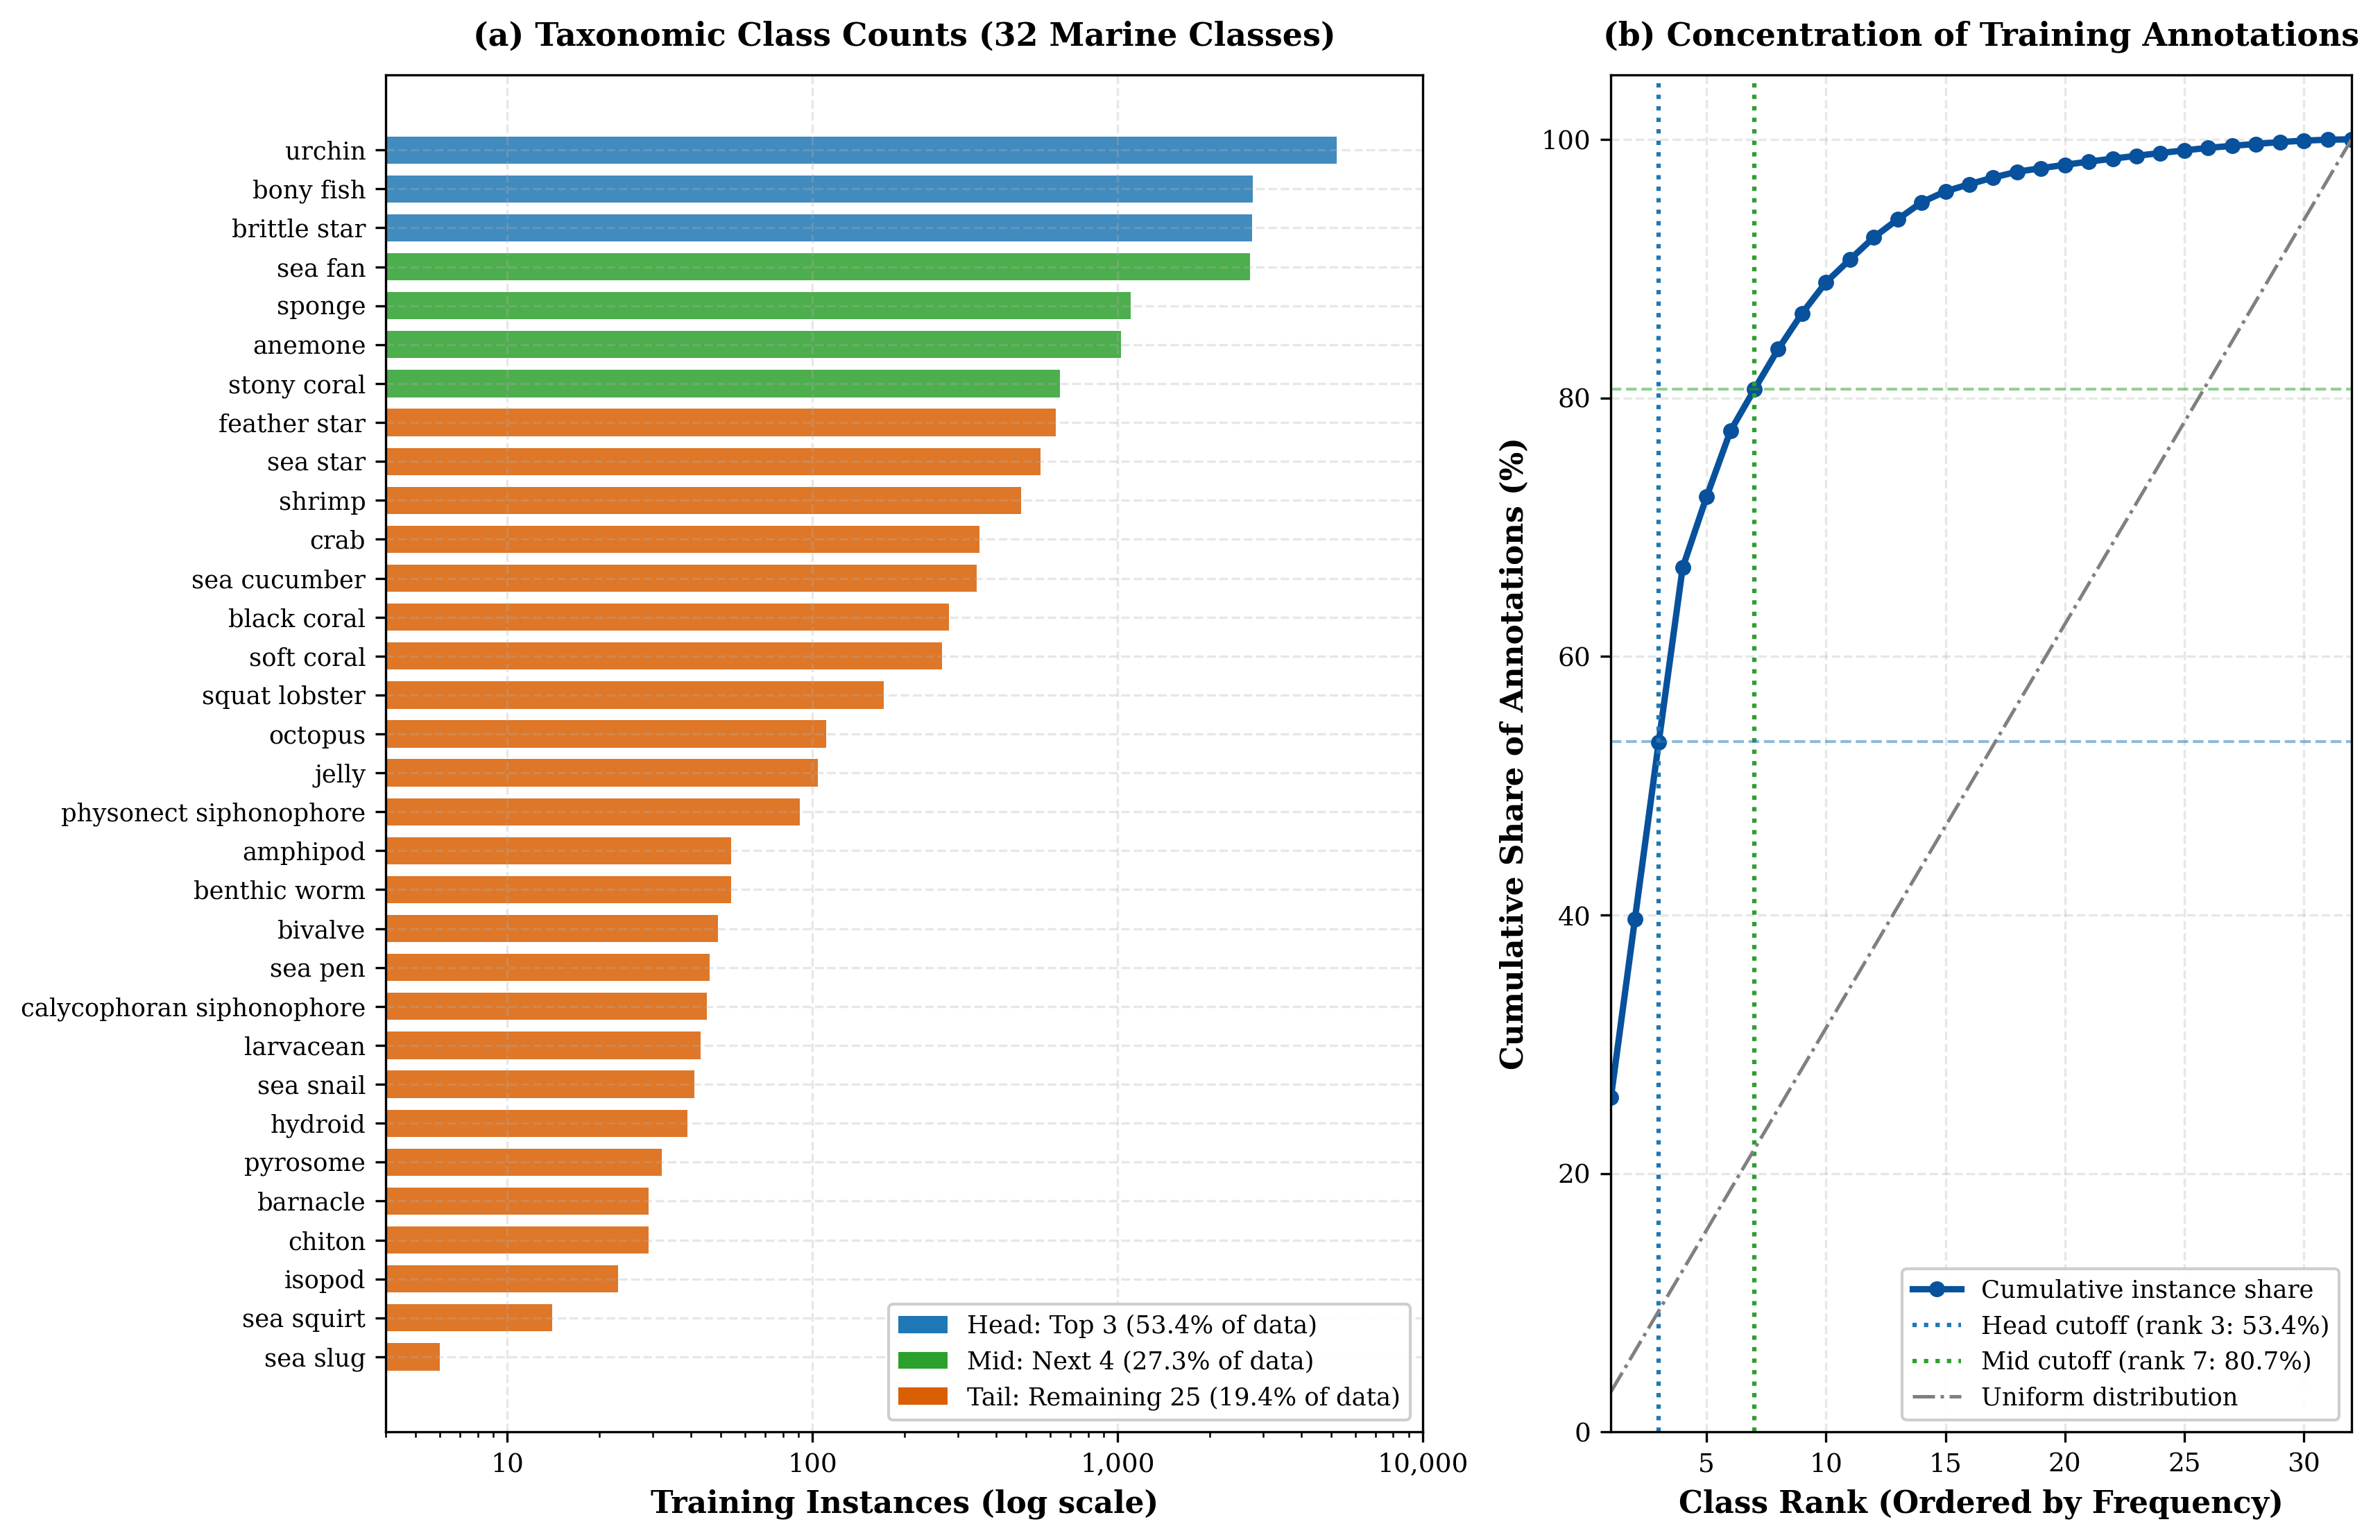
\includegraphics[width=0.75\textwidth]{paper/images/fig_class_imbalance.png}
\caption{Per-class annotation counts in \dataset{}, illustrating the long-tailed distribution. Head classes (bony fish, brittle star, urchin) dominate the annotation count, while most tail classes are represented by only a few dozen instances.}
\label{fig:class-imbalance}
\end{figure}

\subsection{Image and Object Geometry}
Figure~\ref{fig:geometry} summarizes image resolution and object-size statistics. Input images are resized to $640\times640$ pixels for training and evaluation, a common compromise that fits within GPU memory while preserving sufficient detail for medium and large objects. However, many marine organisms --- particularly small invertebrates such as amphipods, isopods, and benthic worms --- occupy a tiny fraction of the image area after resizing. As shown in Section~\ref{sec:results-size}, small objects are effectively undetected at this resolution by all three architectures.

\begin{figure}[H]
\centering
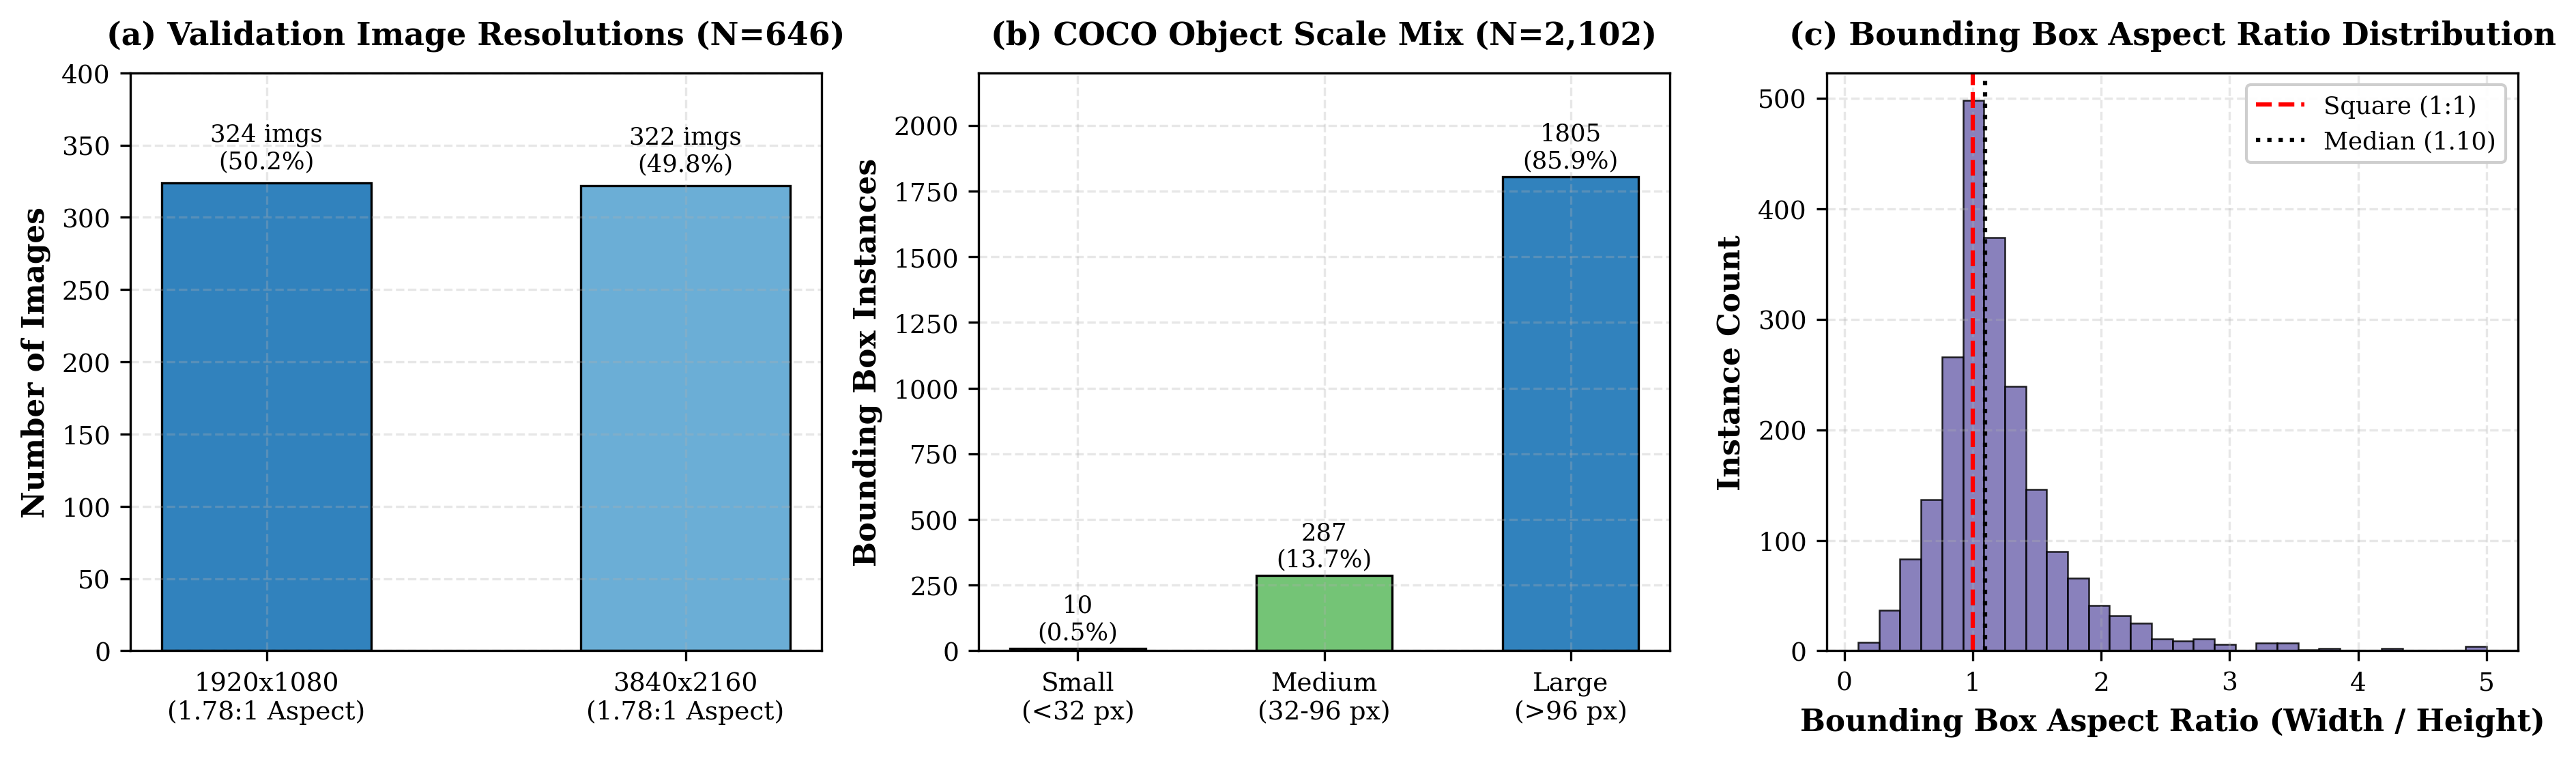
\includegraphics[width=0.75\textwidth]{paper/images/fig_geometry.png}
\caption{Image and object geometry statistics for \dataset{}, including resolution distribution and bounding-box area percentiles.}
\label{fig:geometry}
\end{figure}

\subsection{Split Protocol}
To ensure a fair comparison, all three detectors are trained and evaluated on the same stratified 90/10 image-level train/validation split with random seed 42. Stratification preserves the class distribution across splits, and the split indices are persisted so that every model sees exactly the same data. Evaluation uses COCO-style bounding-box average precision via \texttt{pycocotools}~\cite{pycocotools}, with mAP computed over IoU thresholds $[0.50:0.05:0.95]$ (denoted mAP$_{50\text{-}95}$) and at IoU 0.50 (mAP$_{50}$). The confidence threshold is fixed at $0.001$ and the per-image detection cap at 300 for all models.

% ----------------------------------------------------------------
% 4. METHODS
% ----------------------------------------------------------------
\section{Methods}
\label{sec:methods}

\subsection{Detector Architectures}

\subsubsection{Faster R-CNN R50-FPN (Two-Stage)}
Faster R-CNN~\cite{fasterrcnn2015} with a ResNet-50 backbone and Feature Pyramid Network neck~\cite{fpn2017} is the canonical two-stage detector. In the first stage, a Region Proposal Network proposes candidate object locations; in the second stage, RoIAlign classifies each proposal and refines its bounding box. The two-stage design localizes objects at coarse granularity first, then refines, which often yields superior accuracy on small and cluttered objects at the cost of higher computation and latency. This implementation uses the torchvision/Mask R-CNN lineage~\cite{maskrcnn2017} and is trained in single precision with batch size 2 on a 15~GiB T4 GPU.

\subsubsection{YOLOv8s (One-Stage)}
YOLOv8s~\cite{yolov8_2023} is the small variant of the YOLOv8 one-stage detector family, distributed through the Ultralytics framework~\cite{ultralytics}. It uses an anchor-free detection head, a CSPDarknet-based backbone, and predicts boxes and class probabilities directly from feature maps. One-stage detectors avoid the two-stage propose-then-classify pipeline, making them substantially faster and lighterweight. YOLOv8s has roughly a quarter of the parameters of Faster R-CNN and is mixed-precision trained with batch size 4.

\subsubsection{RT-DETR-L (Transformer-Based)}
RT-DETR~\cite{rtdetr2024} is an end-to-end transformer-based real-time object detector. Building on DETR~\cite{detr2020} and Deformable DETR~\cite{deformable-detr2021}, RT-DETR uses a hybrid efficient encoder and IoU-aware query selection to achieve strong accuracy without NMS. The ``L'' (large) variant evaluated here has the highest parameter count and memory footprint of the three models, requiring mixed-precision training with batch size 4 to fit on the T4 GPU.
\subsection{Experimental Protocol}
\label{sec:methods-training}
All models share the following protocol:
\begin{itemize}[leftmargin=*]
  \item \textbf{Data:} identical stratified 90/10 split, seed 42 (\S\ref{sec:dataset}).
  \item \textbf{Input size:} $640\times640$ pixels.
  \item \textbf{Epochs:} 30 training epochs per model.
  \item \textbf{Evaluation:} COCO mAP via \texttt{pycocotools}, confidence threshold 0.001, max detections 300 per image.
  \item \textbf{Hardware:} NVIDIA T4 GPU, 15~GiB memory.
\end{itemize}

Framework-specific differences (resizing rules, optimizers, augmentation, checkpoint selection) remain, so the results compare representative default training setups rather than strictly equal compute. Training configurations are summarized in Table~\ref{tab:training}.

\begin{table}[H]
\centering
\small
\caption{Training configurations per detector.}
\label{tab:training}
\begin{tabular}{@{}lccc@{}}
\toprule
Configuration & Faster R-CNN & YOLOv8s & RT-DETR-L \\
\midrule
Family & Two-stage & One-stage & Transformer \\
Backbone & R50-FPN & CSPDarknet & Hybrid encoder \\
Batch size & 2 & 4 & 4 \\
Precision & FP32 & Mixed (AMP) & Mixed (AMP) \\
Epochs & 30 & 30 & 30 \\
Input size & $640$ px & $640$ px & $640$ px \\
GPU memory (approx.) & High & Moderate & Highest \\
\bottomrule
\end{tabular}
\end{table}

\subsection{Evaluation Metrics}
The primary metric is COCO mean average precision. mAP$_{50\text{-}95}$ averages AP over IoU thresholds from 0.50 to 0.95 in steps of 0.05, rewarding both localization and classification quality. mAP$_{50}$ uses a single IoU threshold of 0.50 and is more forgiving of localization error. Additional analyses examine per-class AP, head/mid/tail grouping, object-size stratified AP (small/medium/large), and inference latency.

\subsection{Inference Cost Measurement}
Latency is measured on the training hardware (NVIDIA T4) as the median wall-clock time of 30 single-image forward passes at $640\times640$ resolution after five warm-up passes, in batch 1, FP32, from decoded RGB to CPU detections (excluding disk/decode). Parameter counts are taken from the model definitions.

% ----------------------------------------------------------------
% 5. RESULTS
% ----------------------------------------------------------------
\section{Results}
\label{sec:results}

\subsection{Overall Performance}
Table~\ref{tab:main} compares the three detectors on overall accuracy and inference cost. Faster R-CNN R50-FPN is the strongest detector overall, with mAP$_{50\text{-}95}=0.333$ and mAP$_{50}=0.483$. YOLOv8s follows closely at mAP$_{50\text{-}95}=0.313$ and mAP$_{50}=0.428$ (94\% of Faster R-CNN's mAP$_{50\text{-}95}$), while RT-DETR-L trails at mAP$_{50\text{-}95}=0.231$ and mAP$_{50}=0.323$ in this nominally equal configuration.

\begin{table}[H]
\centering
\small
\caption{Overall detection performance and inference cost (median of 30 runs, batch 1, FP32, $640$ px input, NVIDIA T4).}
\label{tab:main}
\begin{tabular}{@{}lcccc@{}}
\toprule
Detector & mAP$_{50\text{-}95}$ & mAP$_{50}$ & mAP$_{75}$ & Latency (ms) \\
\midrule
Faster R-CNN R50-FPN & 0.333 & 0.483 & 0.354 & 46.4 \\
YOLOv8s & 0.313 & 0.428 & 0.356 & 24.0 \\
RT-DETR-L & 0.231 & 0.323 & 0.252 & 62.2 \\
\bottomrule
\end{tabular}
\end{table}

\begin{figure}[H]
\centering
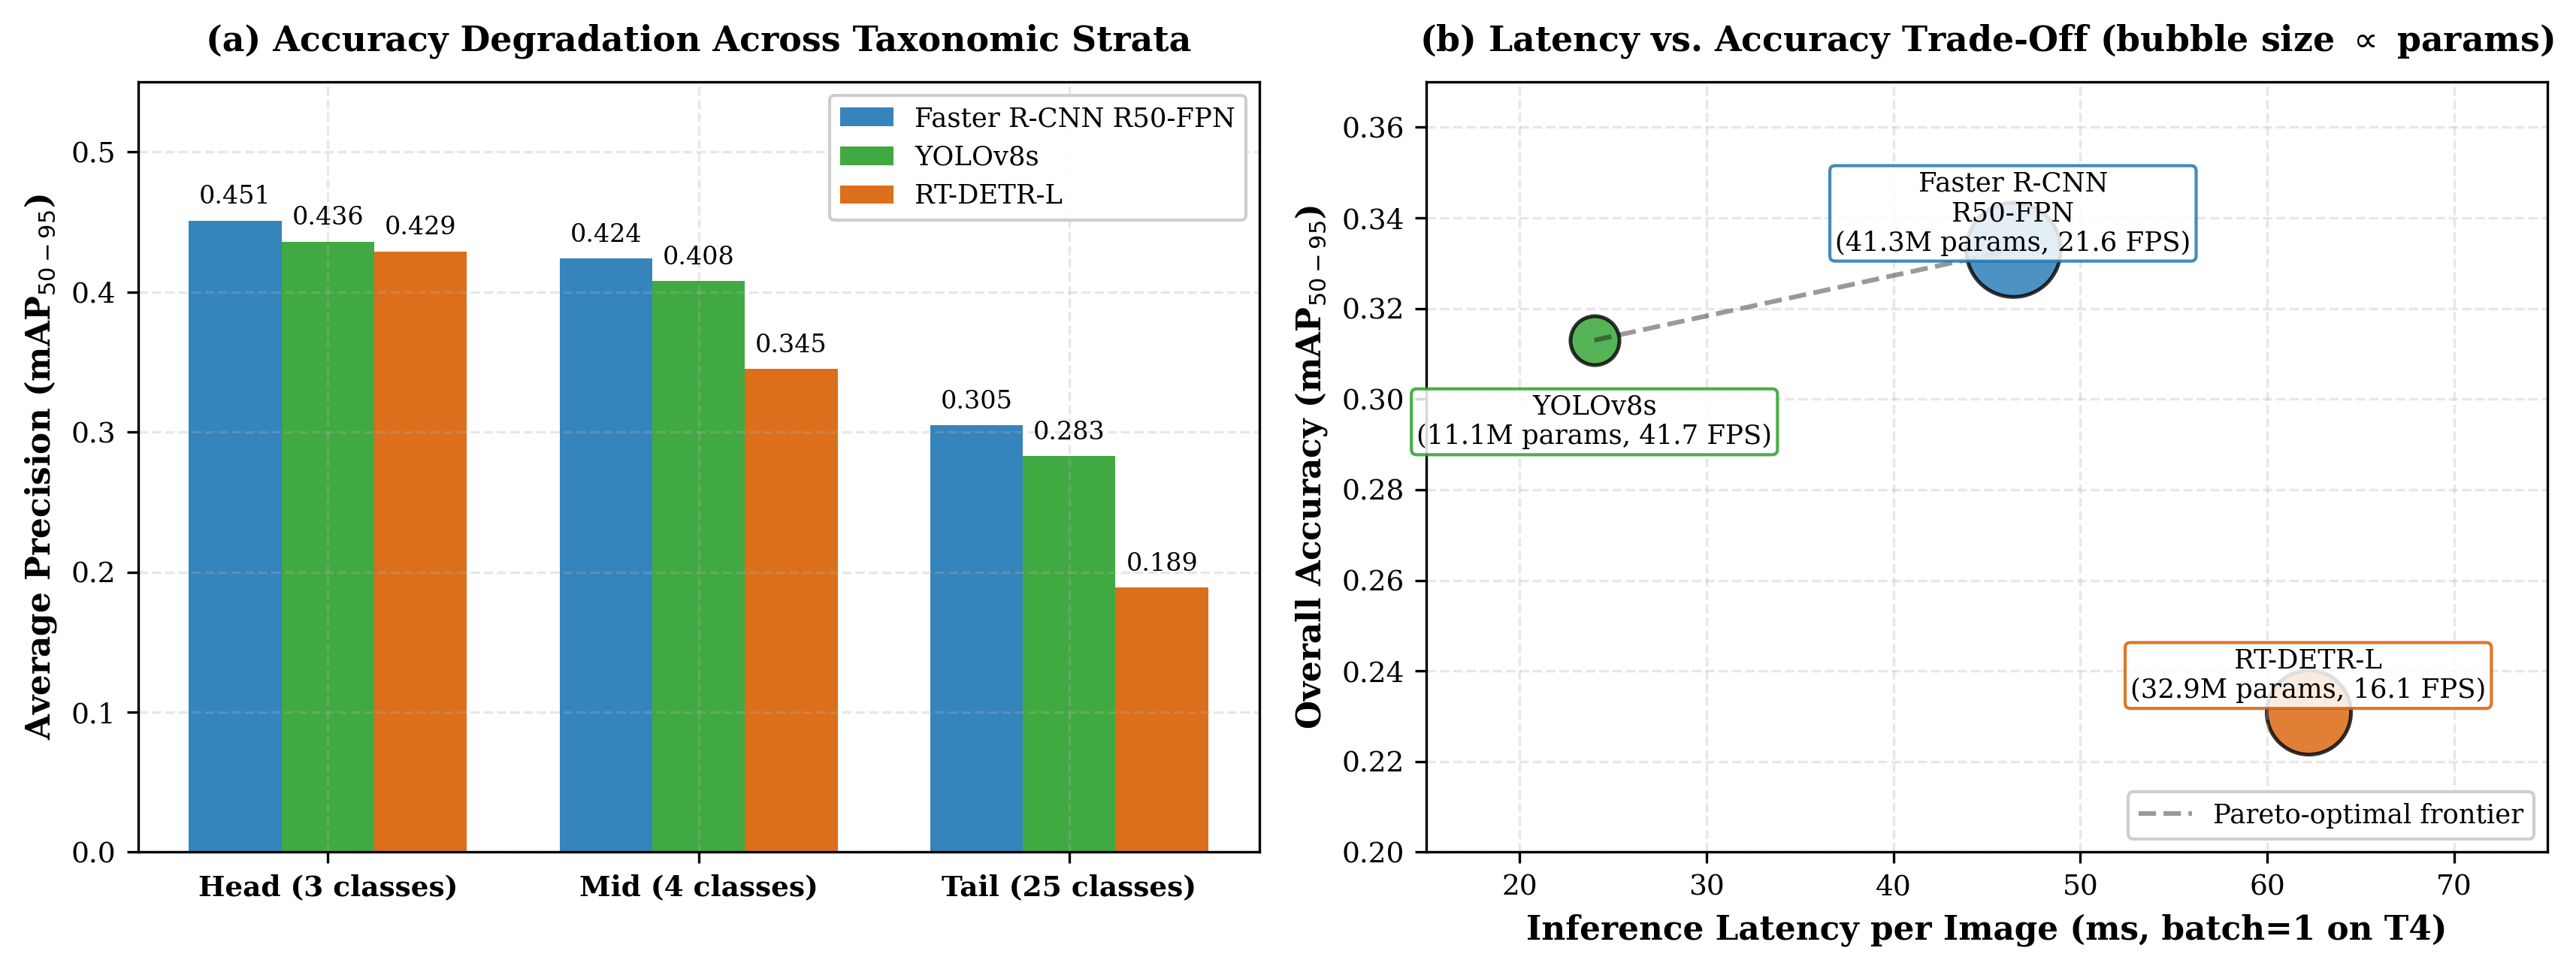
\includegraphics[width=0.70\textwidth]{paper/images/fig_performance_tradeoff.png}
\caption{Accuracy--latency trade-off across the three detectors. Faster R-CNN leads in accuracy; YOLOv8s offers the best accuracy--cost balance; RT-DETR-L is neither the most accurate nor the fastest in this configuration.}
\label{fig:perf-tradeoff}
\end{figure}

Figure~\ref{fig:perf-tradeoff} visualizes the trade-off. YOLOv8s reaches $94\%$ of Faster R-CNN's mAP$_{50\text{-}95}$ at roughly 52\% of its latency and with approximately one quarter of the parameters, making it attractive for deployment on resource-constrained underwater vehicles. RT-DETR-L is the slowest ($62.2$ ms/image) and least accurate in this setup, so it is best viewed as the transformer-family baseline rather than a deployment recommendation from these runs.

\subsection{Training Curves}
Figure~\ref{fig:curves} shows the validation mAP$_{50\text{-}95}$ training curves for all three detectors over 30 epochs. Faster R-CNN and YOLOv8s both converge steadily, while RT-DETR-L exhibits a slower and noisier learning trajectory consistent with the known data-hunger and convergence challenges of end-to-end transformers.

\begin{figure}[H]
\centering
\begin{subfigure}{0.32\textwidth}
\centering
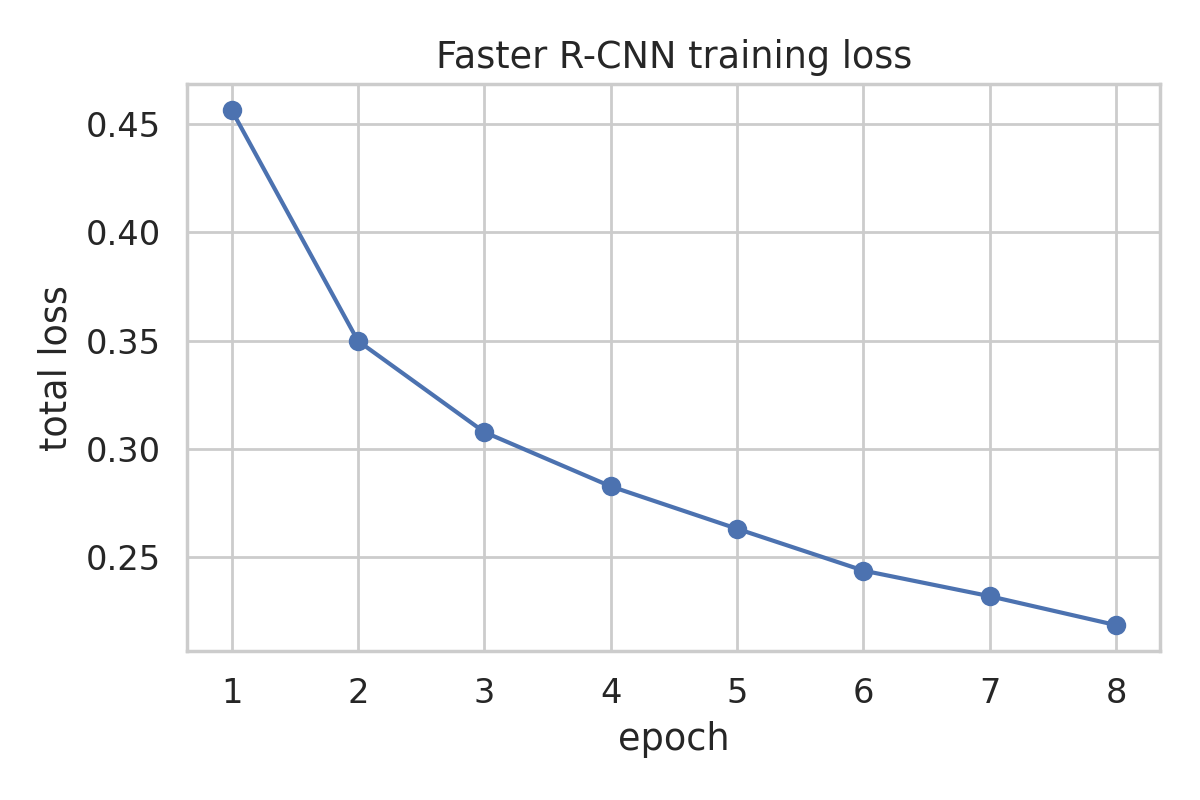
\includegraphics[width=\textwidth]{paper/images/curve_fasterrcnn.png}
\caption{Faster R-CNN}
\end{subfigure}%
\begin{subfigure}{0.32\textwidth}
\centering
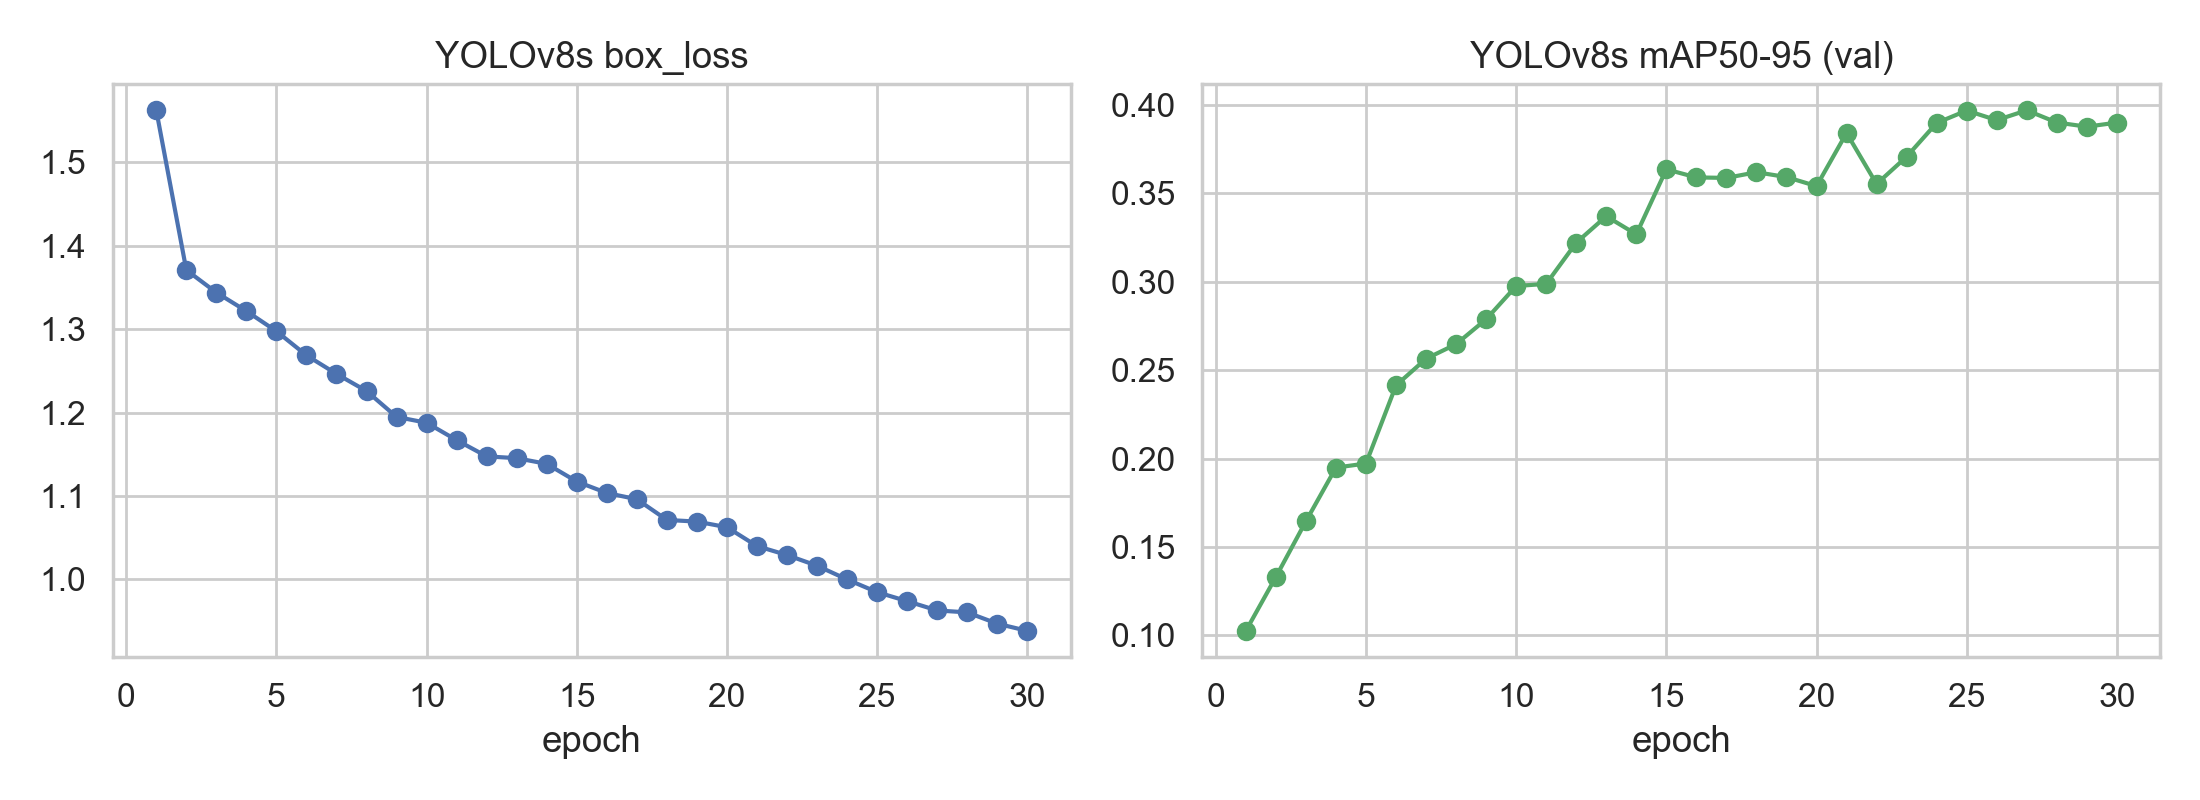
\includegraphics[width=\textwidth]{paper/images/curve_yolov8s.png}
\caption{YOLOv8s}
\end{subfigure}%
\begin{subfigure}{0.32\textwidth}
\centering
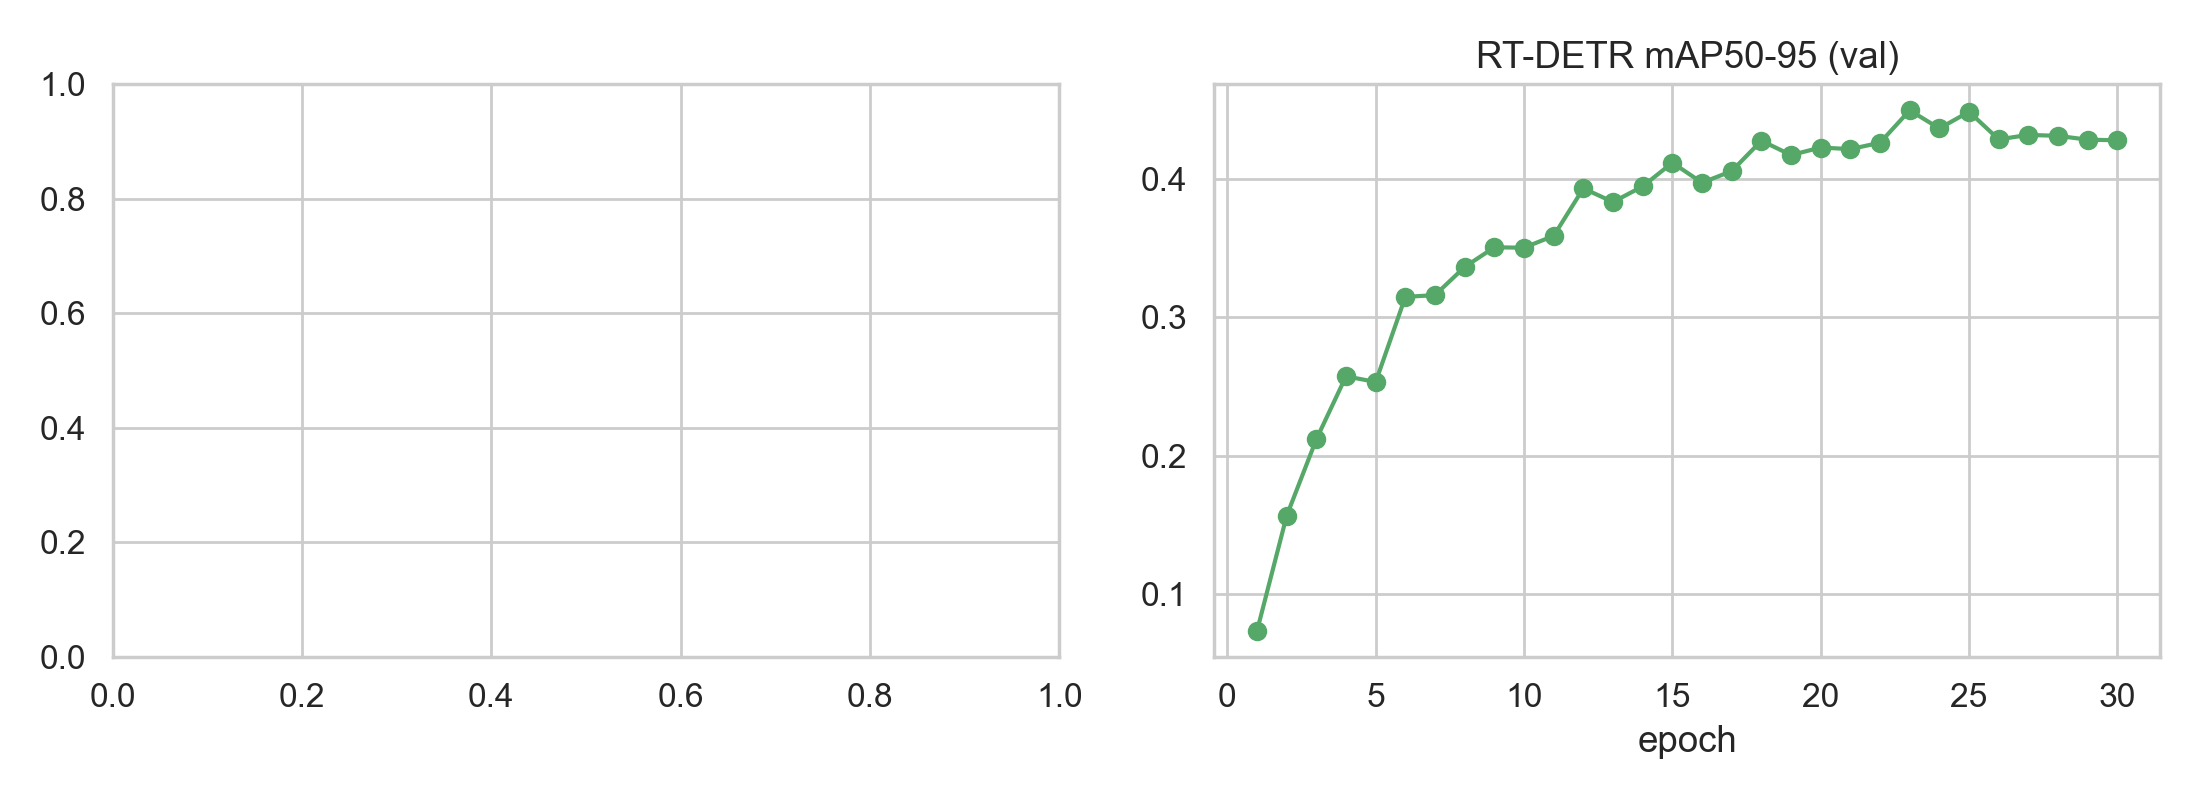
\includegraphics[width=\textwidth]{paper/images/curve_rtdetr.png}
\caption{RT-DETR-L}
\end{subfigure}
\caption{Validation mAP$_{50\text{-}95}$ training curves over 30 epochs for each detector (identical data split).}
\label{fig:curves}
\end{figure}
\subsection{Per-Class Analysis}
\label{sec:results-perclass}
Table~\ref{tab:perclass} reports per-class AP$_{50\text{-}95}$ for Faster R-CNN (the strongest detector), with representative values. Classes separate into clear tiers: easy classes (pyrosome, larvacean, hydroid, urchin, stony coral) achieve AP above 0.55, medium classes (anemone, sea fan, sponge, crab, octopus) lie in the 0.2--0.4 range, and hard tail classes (amphipod, bivalve, sea slug, sea squirt, barnacle) approach zero. The same ordering holds qualitatively for YOLOv8s and RT-DETR-L, confirming that per-class difficulty is driven primarily by the data distribution (annotation count and object size) rather than by architecture.

\begin{table}[H]
\centering
\small
\caption{Per-class AP$_{50\text{-}95}$ for Faster R-CNN R50-FPN (selected classes; full table in Appendix~\ref{app:perclass}).}
\label{tab:perclass}
\begin{tabular}{@{}lcc@{}}
\toprule
Class & AP$_{50\text{-}95}$ & Group \\
\midrule
pyrosome & 0.925 & tail \\
larvacean & 0.718 & tail \\
hydroid & 0.653 & tail \\
urchin & 0.592 & head \\
stony coral & 0.586 & mid \\
soft coral & 0.563 & tail \\
crab & 0.517 & tail \\
bony fish & 0.464 & head \\
barnacle & 0.454 & tail \\
anemone & 0.309 & mid \\
sea fan & 0.405 & mid \\
sponge & 0.397 & mid \\
brittle star & 0.297 & head \\
sea cucumber & 0.268 & tail \\
benthic worm & 0.001 & tail \\
amphipod & 0.000 & tail \\
bivalve & 0.000 & tail \\
sea slug & 0.000 & tail \\
sea squirt & 0.000 & tail \\
\bottomrule
\end{tabular}
\end{table}

Table~\ref{tab:hmt} aggregates performance by head/mid/tail grouping. All three detectors show a consistent degradation from head to tail: head AP$_{50\text{-}95}$ ranges from 0.43--0.45, mid from 0.35--0.42, and tail from 0.19--0.30. This gradient is inherited directly from the long-tailed annotation distribution shown in Figure~\ref{fig:class-imbalance}.

\subsection{Object-Size Analysis}
\label{sec:results-size}
Table~\ref{tab:size} reports size-stratified AP$_{50\text{-}95}$ (small/medium/large). Large objects are detected with moderate accuracy (0.25--0.38), medium objects poorly (0.06--0.08), and small objects effectively not at all (0.00--0.01). This reflects the $640\times640$ input resolution, under which many small marine invertebrates occupy only a few pixels. Addressing small-object detection would require higher-resolution inputs, test-time tiling, or dedicated small-object augmentation --- directions left for future work.

\begin{table}[H]
\centering
\small
\caption{Size-stratified AP$_{50\text{-}95}$ by detector at $640$ px input.}
\label{tab:size}
\begin{tabular}{@{}lccc@{}}
\toprule
Detector & Small & Medium & Large \\
\midrule
Faster R-CNN R50-FPN & 0.007 & 0.059 & 0.377 \\
YOLOv8s & 0.000 & 0.063 & 0.350 \\
RT-DETR-L & 0.000 & 0.075 & 0.254 \\
\bottomrule
\end{tabular}
\end{table}

\subsection{Inference Cost}
YOLOv8s is the fastest detector at $24.0$ ms per image, Faster R-CNN intermediate at $46.4$ ms, and RT-DETR-L slowest at $62.2$ ms. For on-platform deployment, the trade-off is clear: Faster R-CNN is the accuracy leader but costs $1.9\times$ the latency of YOLOv8s; YOLOv8s reaches 94\% of Faster R-CNN's mAP$_{50\text{-}95}$ at roughly half the latency with far fewer parameters and fits comfortably on a 15~GiB GPU alongside the rest of a vehicle software stack. Memory constraints are significant: both Ultralytics runs used mixed precision with batch 4, while Faster R-CNN used batch 2 in single precision; larger batches or higher resolutions would exceed a single commodity GPU.
\subsection{Qualitative Results}
Figure~\ref{fig:qualitative} presents matched qualitative detection panels across the three architectures on representative validation frames at a score threshold of 0.25, with ground-truth boxes overlaid. Panels are drawn from the easiest classes (urchin, pyrosome) and the hardest (sea slug, amphipod). Detections on easy, large, frequent classes are consistent across all detectors; on rare, small, or camouflaged taxa, detections are sparse or absent even for the best model.

\begin{figure}[H]
\centering
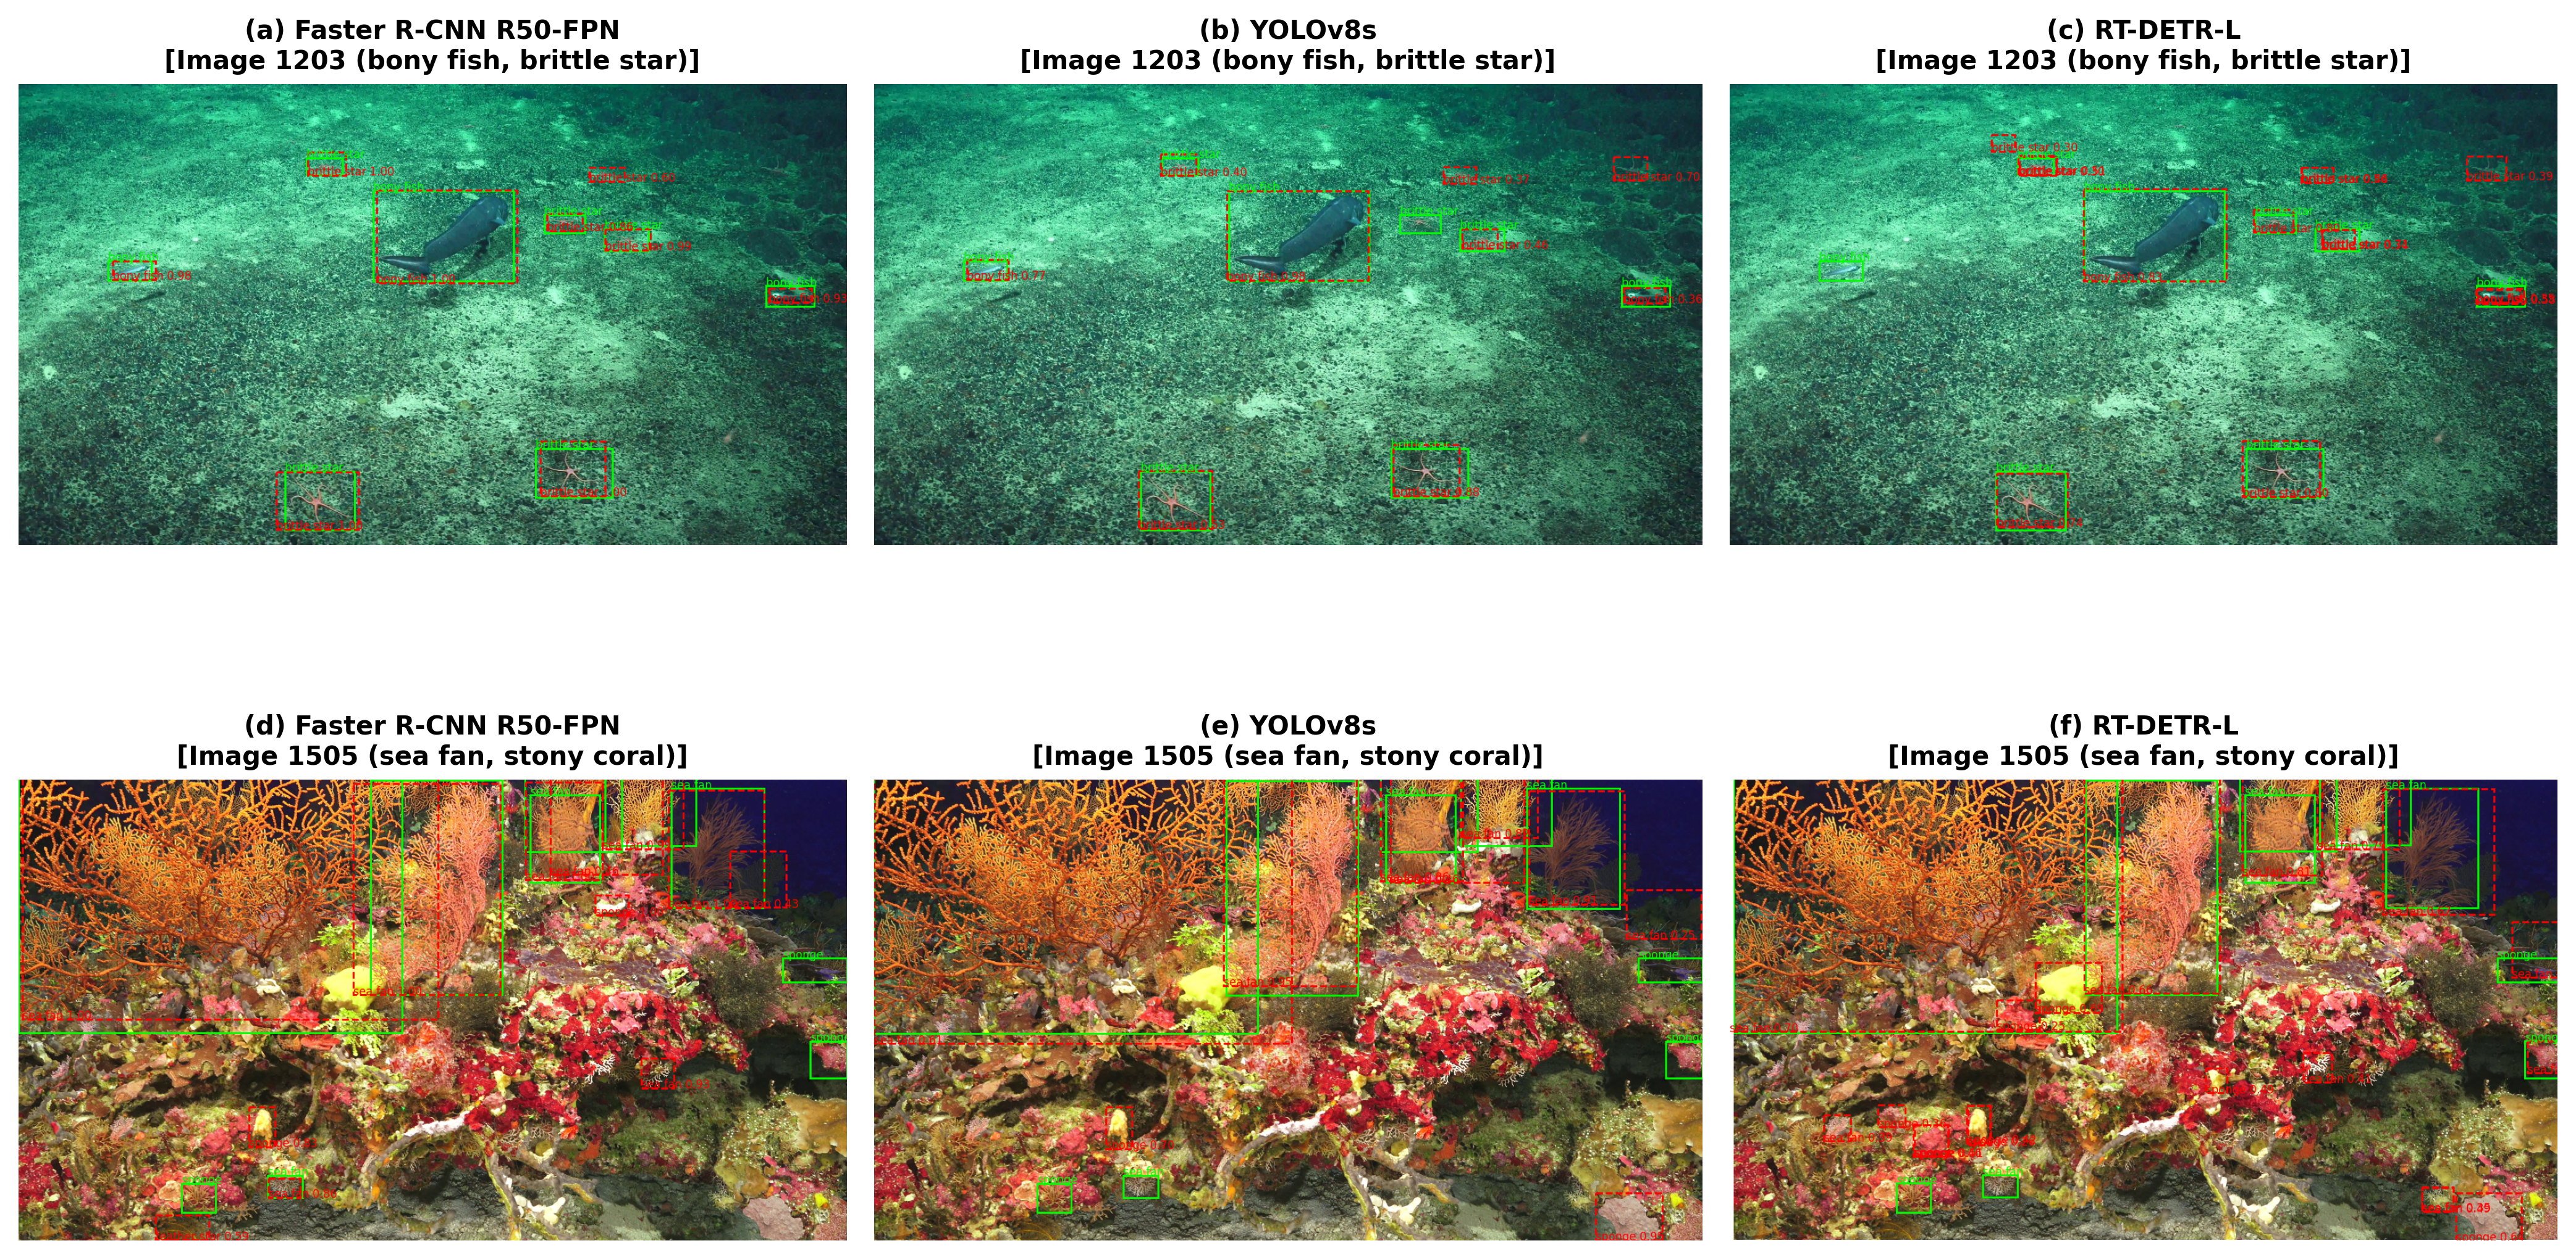
\includegraphics[width=0.85\textwidth]{paper/images/fig_qualitative_large.png}
\caption{Qualitative detection panels for Faster R-CNN, YOLOv8s, and RT-DETR-L on representative validation frames (ground truth overlaid, score threshold 0.25).}
\label{fig:qualitative}
\end{figure}

\subsection{Grad-CAM Analysis}
Figure~\ref{fig:gradcam} shows high-resolution Grad-CAM visual attributions on the same scenes, comparing feature-activation patterns across deep network layers. The attention maps confirm that detectors focus on salient foreground regions for easy classes, while activations are diffuse or absent for hard tail classes --- consistent with the quantitative per-class results.

\begin{figure}[H]
\centering
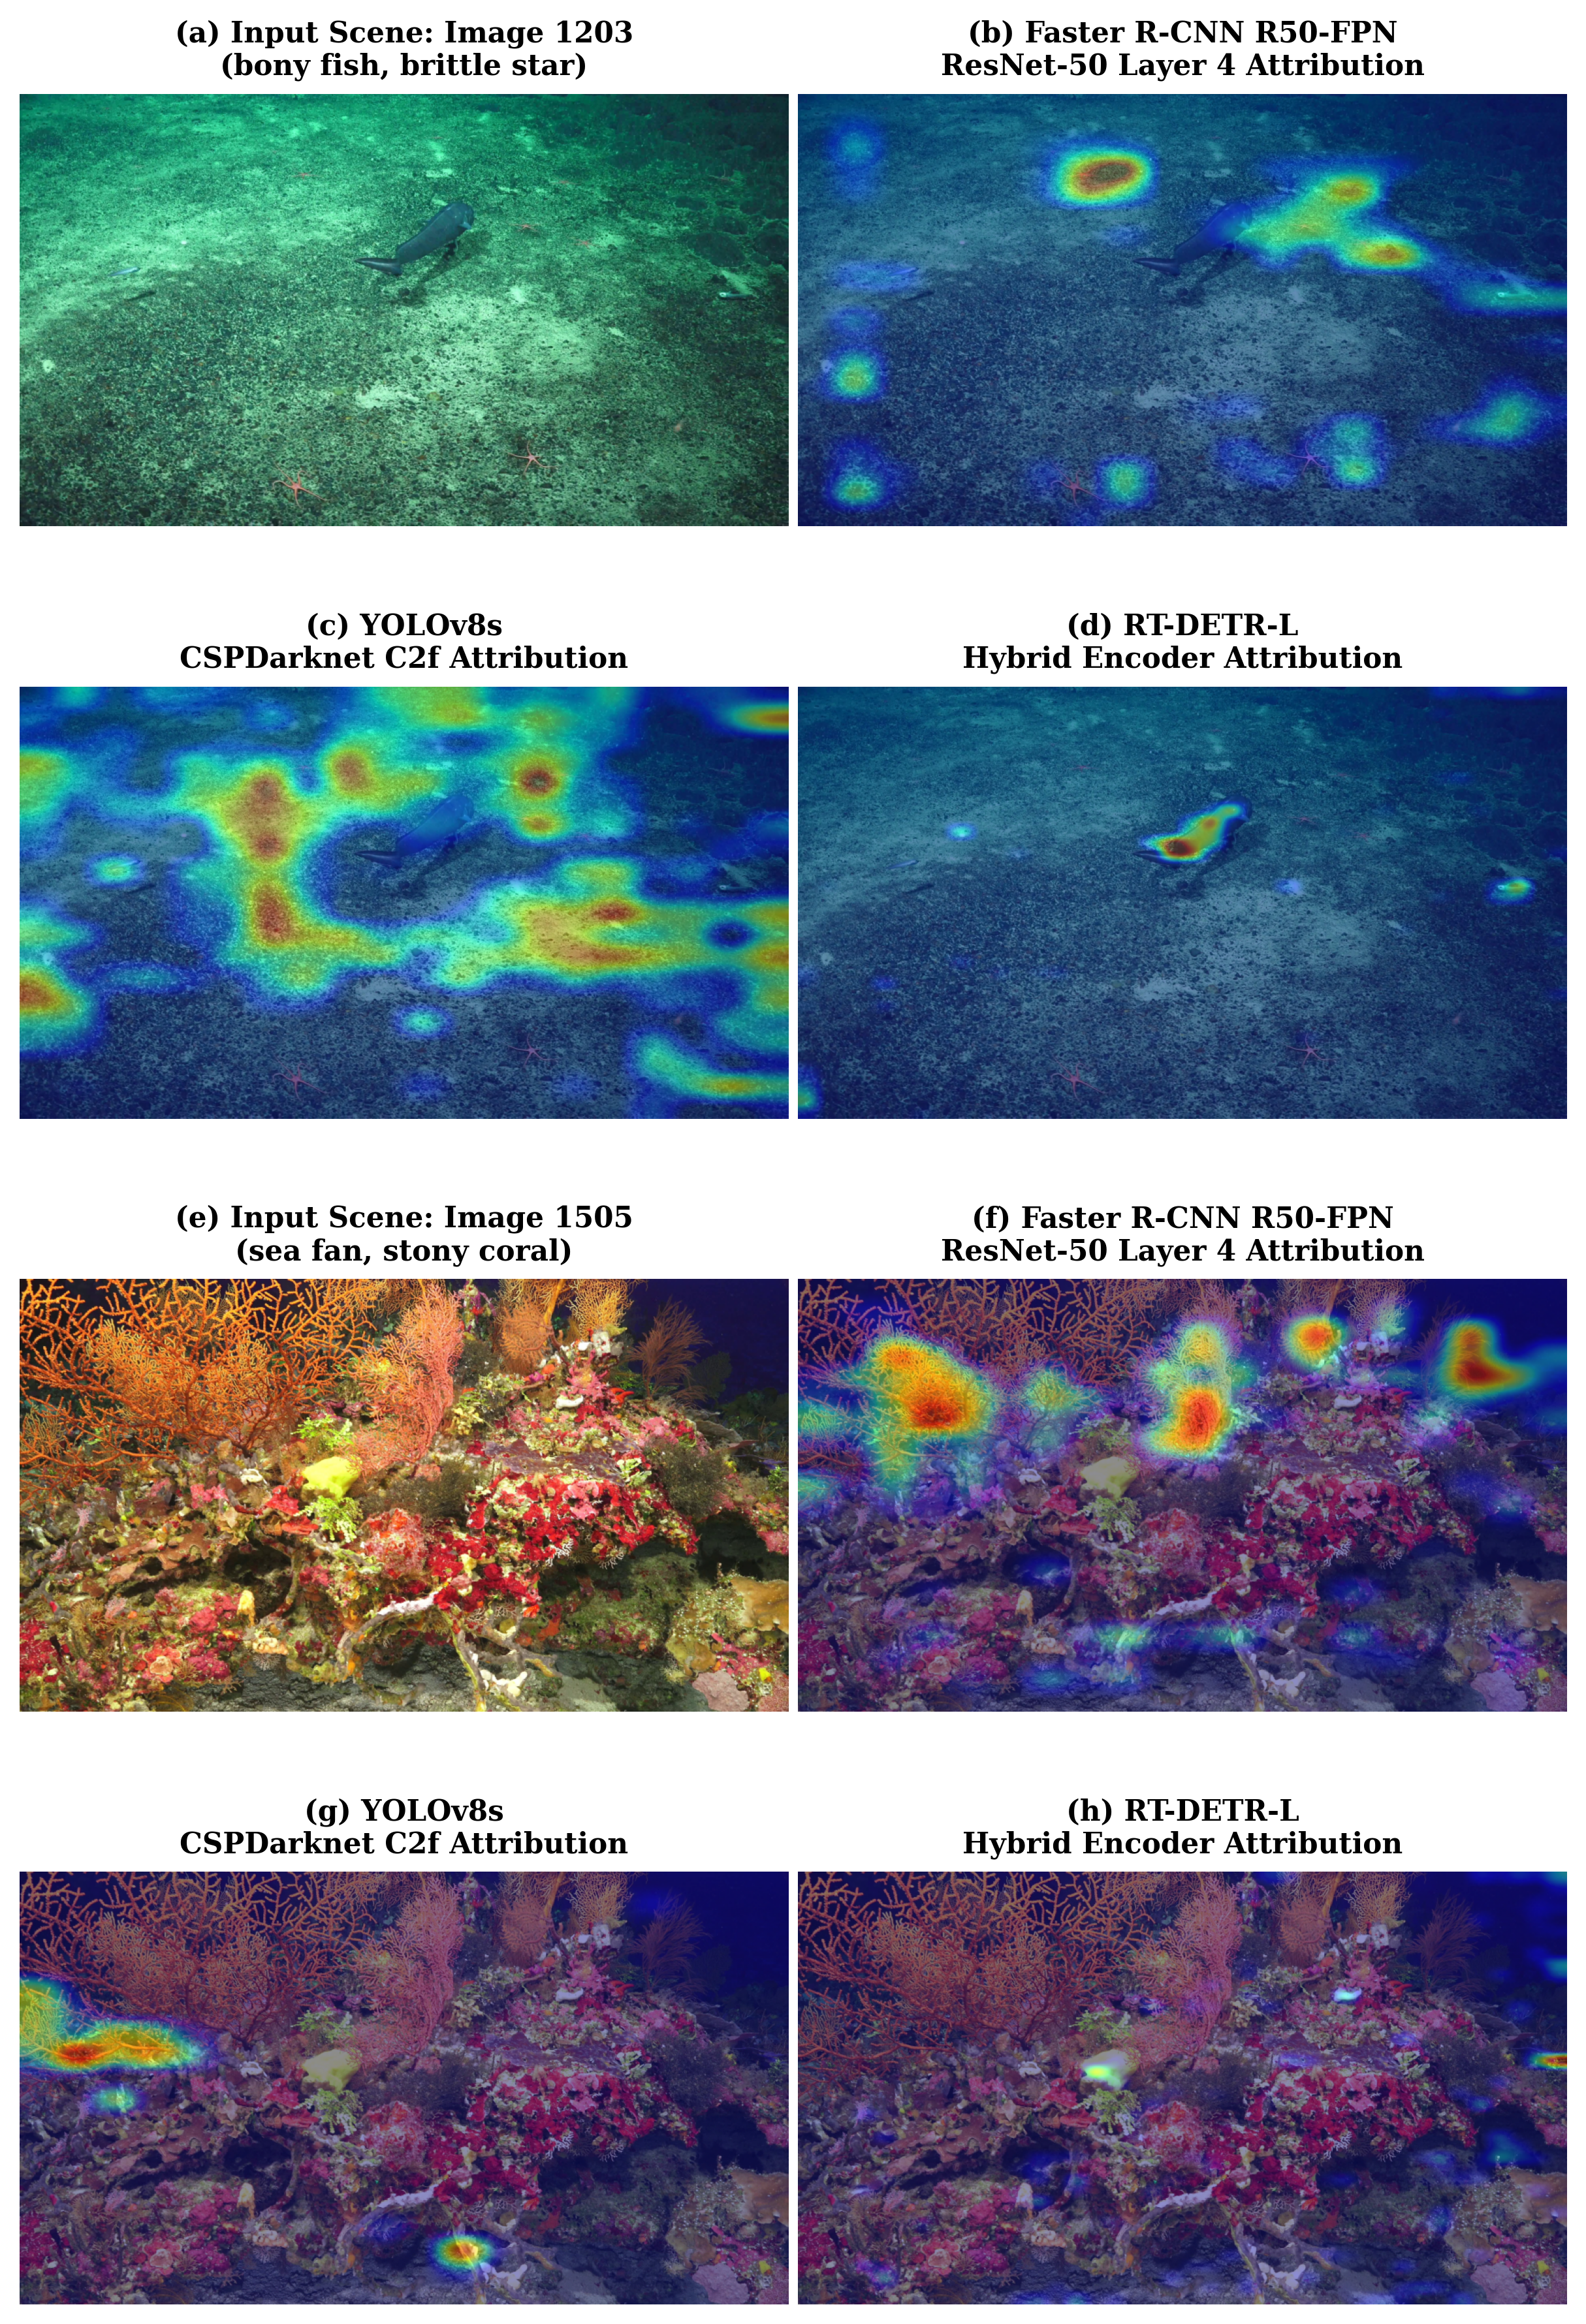
\includegraphics[width=0.85\textwidth]{paper/images/fig_gradcam_large.png}
\caption{Grad-CAM visual attributions comparing feature activation across network layers for the three detectors.}
\label{fig:gradcam}
\end{figure}

% ----------------------------------------------------------------
% 6. DISCUSSION
% ----------------------------------------------------------------
\section{Discussion}
\label{sec:discussion}

The observed ranking --- two-stage $>$ one-stage $>$ transformer in this nominally equal 30-epoch, 640 px configuration --- must be read with the configuration caveat of Section~\ref{sec:methods-training}. All runs share the split, confidence threshold, detection cap, and nominal epoch/resolution budget, but framework-specific resizing rules, optimizers, augmentation, and checkpoint-selection rules differ; hence these numbers compare representative default training setups rather than a strictly controlled compute comparison. The head-to-tail degradation shared by all three runs is nevertheless inherited directly from the data distribution, and the per-class pattern is consistent across families.

For deployment on ROV/AUV platforms, YOLOv8s sits at the sweet spot of the accuracy--cost curve: near-Faster R-CNN accuracy at roughly half the latency and one quarter of the parameters, with modest memory requirements. Faster R-CNN is the accuracy ceiling in this configuration and remains preferable when inference latency is secondary to detection quality (e.g., offline post-processing of collected imagery). RT-DETR-L is neither the most accurate nor the fastest here and is best regarded as the transformer-family baseline; its relatively high memory footprint also makes it less attractive on single-GPU embedded platforms unless further optimized (distillation, quantization, smaller variant).

Which findings transfer? The head-to-tail degradation ordering should generalize to any long-tailed underwater dataset, since it reflects annotation frequency and object scale rather than architecture. The small-object blind spot at 640 px should also transfer across architectures and datasets. Exact mAP values, of course, are dataset- and protocol-specific.

% ----------------------------------------------------------------
% 7. LIMITATIONS
% ----------------------------------------------------------------
\section{Limitations}
\label{sec:limitations}

\begin{enumerate}[leftmargin=*]
  \item \textbf{Single split and seed.} Results are based on one stratified 90/10 split (seed 42); multi-seed variance is not reported.
  \item \textbf{Validation-only evaluation.} No blind test-set results are reported; all numbers are on the validation split.
  \item \textbf{Nominally equal, not identical, compute.} Framework-specific augmentation, optimizer, and checkpoint-selection rules differ across detectors.
  \item \textbf{Single hardware.} Latency and memory measurements are specific to the NVIDIA T4 (15~GiB).
  \item \textbf{Modest training budget.} All models train for 30 epochs; longer schedules, larger batches, or higher resolutions were not feasible within the memory and time constraints.
  \item \textbf{No algorithmic long-tailed intervention.} Standard cross-entropy training is used throughout; class-balanced losses, resampling, or pseudo-labeling were not explored.
\end{enumerate}

% ----------------------------------------------------------------
% 8. CONCLUSION
% ----------------------------------------------------------------
\section{Conclusion and Future Work}
\label{sec:conclusion}

This report benchmarks Faster R-CNN R50-FPN, YOLOv8s, and RT-DETR-L on \dataset{} underwater imagery under a controlled protocol. Faster R-CNN achieves the best accuracy (mAP$_{50\text{-}95}=0.333$), YOLOv8s offers the best accuracy--latency trade-off (mAP$_{50\text{-}95}=0.313$ at 24 ms/image), and RT-DETR-L trails in this configuration (mAP$_{50\text{-}95}=0.231$ at 62 ms/image). All detectors exhibit strong head-to-tail degradation driven by the long-tailed class distribution, and small objects are effectively undetected at $640$ px resolution.

For practical AUV/ROV deployment, YOLOv8s is the recommended starting point; Faster R-CNN is the accuracy ceiling when latency is less critical. Future work includes: longer training schedules and multi-seed evaluation; test-time tiling and higher-resolution inputs for small objects; long-tailed losses and resampling; model compression (quantization, distillation) for embedded deployment; and blind test-set submission to the \dataset{} challenge.

% ----------------------------------------------------------------
% APPENDIX
% ----------------------------------------------------------------
\appendix
\onecolumn

\section{Full Per-Class AP Table}
\label{app:perclass}
Table~\ref{tab:perclass-full} reports the complete per-class AP$_{50\text{-}95}$ for Faster R-CNN R50-FPN across all 32 classes.

\begin{table}[H]
\centering
\small
\caption{Full per-class AP$_{50\text{-}95}$ for Faster R-CNN R50-FPN.}
\label{tab:perclass-full}
\begin{tabular}{@{}lc@{}}
\toprule
Class & AP$_{50\text{-}95}$ \\
\midrule
amphipod & 0.000 \\
anemone & 0.309 \\
barnacle & 0.454 \\
benthic worm & 0.001 \\
bivalve & 0.000 \\
black coral & 0.246 \\
bony fish & 0.464 \\
brittle star & 0.297 \\
calycophoran siphonophore & 0.200 \\
chiton & 0.443 \\
crab & 0.517 \\
feather star & 0.354 \\
hydroid & 0.653 \\
isopod & 0.078 \\
jelly & 0.140 \\
larvacean & 0.718 \\
octopus & 0.426 \\
physonect siphonophore & 0.528 \\
pyrosome & 0.925 \\
sea cucumber & 0.268 \\
sea fan & 0.405 \\
sea pen & 0.222 \\
sea slug & 0.000 \\
sea snail & 0.167 \\
sea squirt & 0.000 \\
sea star & 0.267 \\
shrimp & 0.205 \\
soft coral & 0.563 \\
sponge & 0.397 \\
squat lobster & 0.238 \\
stony coral & 0.586 \\
urchin & 0.592 \\
\bottomrule
\end{tabular}
\end{table}

\section{Head/Mid/Tail and Size AP by Detector}
\label{app:grouping}
Tables~\ref{tab:hmt} and~\ref{tab:size-full} summarize head/mid/tail and size-stratified results for all detectors.

\begin{table}[H]
\centering
\small
\caption{Head/mid/tail AP$_{50\text{-}95}$ by detector.}
\label{tab:hmt}
\begin{tabular}{@{}lccc@{}}
\toprule
Detector & Head & Mid & Tail \\
\midrule
Faster R-CNN R50-FPN & 0.451 & 0.424 & 0.305 \\
YOLOv8s & 0.436 & 0.408 & 0.283 \\
RT-DETR-L & 0.429 & 0.345 & 0.189 \\
\bottomrule
\end{tabular}
\end{table}

\begin{table}[H]
\centering
\small
\caption{Size-stratified AP$_{50\text{-}95}$ by detector.}
\label{tab:size-full}
\begin{tabular}{@{}lccc@{}}
\toprule
Detector & Small & Medium & Large \\
\midrule
Faster R-CNN R50-FPN & 0.007 & 0.059 & 0.377 \\
YOLOv8s & 0.000 & 0.063 & 0.350 \\
RT-DETR-L & 0.000 & 0.075 & 0.254 \\
\bottomrule
\end{tabular}
\end{table}

\section{Hardware and Software}
\label{app:repro}
Experiments were run on Kaggle using an NVIDIA T4 GPU with 15~GiB memory. The software stack comprises Python 3.9+, PyTorch~\cite{paszke2019pytorch}, torchvision, \texttt{pycocotools}~\cite{pycocotools}, Albumentations, OpenCV, and Ultralytics~\cite{ultralytics}. Code is organized under \texttt{src/} (data loading, detector wrappers, training and evaluation utilities) with experiment configs in \texttt{configs/} and Kaggle training notebooks under \texttt{notebooks/kaggle/}. All runs share split \texttt{split\_fingerprint = d611d16e1c9c0562}, score threshold 0.001, and max detections 300.

% ----------------------------------------------------------------
% REFERENCES
% ----------------------------------------------------------------
\begin{thebibliography}{99}

\bibitem{fathomnet2022}
K.~Katija et al., ``FathomNet: A global image database for enabling artificial intelligence in the ocean,'' \emph{Scientific Reports}, vol.~12, no.~1, p.~15914, 2022. \url{https://doi.org/10.1038/s41598-022-19939-2}

\bibitem{fathomnet-clef-2026}
FathomNet CLEF 2026 Organizers, ``FathomNet CLEF 2026: ImageCLEF LifeCLEF track on underwater object detection,'' 2026. \url{https://www.imageclef.org/}

\bibitem{fathomnet-2021-workshop}
O.~Boulais et al., ``FathomNet: An underwater image training database for ocean exploration and discovery,'' \emph{arXiv preprint arXiv:2007.00114}, 2020.

\bibitem{coco2014}
T.-Y. Lin et al., ``Microsoft COCO: Common Objects in Context,'' in \emph{ECCV}, pp.~740--755, 2014.

\bibitem{pycocotools}
COCO Dataset Organizers, ``pycocotools: Official COCO API.'' \url{https://github.com/cocodataset/cocoapi}

\bibitem{fasterrcnn2015}
S.~Ren, K.~He, R.~Girshick, and J.~Sun, ``Faster R-CNN: Towards Real-Time Object Detection with Region Proposal Networks,'' in \emph{NeurIPS}, vol.~28, pp.~91--99, 2015.

\bibitem{fpn2017}
T.-Y. Lin et al., ``Feature Pyramid Networks for Object Detection,'' in \emph{CVPR}, pp.~936--944, 2017.

\bibitem{maskrcnn2017}
K.~He et al., ``Mask R-CNN,'' in \emph{ICCV}, pp.~2980--2988, 2017.

\bibitem{yolov8_2023}
Ultralytics, ``YOLOv8,'' 2023. \url{https://github.com/ultralytics/ultralytics}

\bibitem{ultralytics}
Ultralytics, ``Ultralytics Python Package,'' 2023. \url{https://github.com/ultralytics/ultralytics}

\bibitem{detr2020}
N.~Carion et al., ``End-to-End Object Detection with Transformers,'' in \emph{ECCV}, pp.~213--229, 2020.

\bibitem{deformable-detr2021}
X.~Zhu et al., ``Deformable DETR: Deformable Transformers for End-to-End Object Detection,'' in \emph{ICLR}, 2021.

\bibitem{rtdetr2024}
Y.~Zhao et al., ``DETRs Beat YOLOs on Real-time Object Detection,'' in \emph{CVPR}, pp.~16965--16974, 2024.

\bibitem{underwater-survey}
L.~Chen et al., ``Underwater Object Detection in the Era of Artificial Intelligence: Current, Challenge, and Future,'' \emph{arXiv preprint arXiv:2410.05577}, 2024.

\bibitem{paszke2019pytorch}
A.~Paszke et al., ``PyTorch: An Imperative Style, High-Performance Deep Learning Library,'' in \emph{NeurIPS}, vol.~32, pp.~8024--8035, 2019.

\bibitem{kaggle}
Kaggle, ``Kaggle: Your Machine Learning and Data Science Community,'' 2026. \url{https://www.kaggle.com/}

\end{thebibliography}

\end{document}